% !TeX root = main.tex

\documentclass[11pt]{article}

\usepackage[utf8]{inputenc}
\usepackage{amsmath, amssymb}
\usepackage{geometry}
\usepackage{graphicx}
\usepackage{tikz}
\usepackage{hyperref}
\usepackage{enumitem}
\usepackage{titlesec}
\usepackage{float}


\usepackage{booktabs}
\usepackage{threeparttable}
\usetikzlibrary{arrows.meta, positioning}

\geometry{margin=1in}
\titleformat{\section}[block]{\large\bfseries}{\thesection}{1em}{}
\titleformat{\subsection}[block]{\normalsize\bfseries}{\thesubsection}{1em}{}

% === Metadata === \today
\title{LLM Benchmarking Framework for Description Logic Reasoning}
\author{Phanphum Prathumsuwan\\Mahidol University\\phanphum.pra@student.mahidol.ac.th}
\date{August 19, 2025}

\begin{document}

\maketitle

% --- Abstract ---
\begin{abstract}
This paper presents a novel benchmarking framework to evaluate the Description Logic (DL) reasoning capabilities of Large Language Models (LLMs). 
While prior work has tested LLMs on symbolic reasoning and natural language inference\cite{leapofthought2020,han2022folio}, few have focused on the structured semantics of DL, particularly the EL and ELH fragments widely used in ontology engineering\cite{baader2005el}. 
The framework extracts EL axioms from the Pizza ontology\cite{stanford2025pizza, horridge2004pizza} and extends them with role inclusion to create ELH-compliant cases, thereby increasing DL complexity. It then generates corresponding natural language queries, and compares model responses to formal entailment outcomes using the OWL API\cite{owlapi} and HermiT reasoner\cite{hermit2007, glimm2014hermit}. 
We evaluate seven LLMs, including GPT-4o\cite{gpt4o}, Gemini 2.5 Pro\cite{gemini}, LLaMA 3\cite{llama3}, and Gemma 2\cite{gemma3}, Mistral\cite{mistral}, Qwen\cite{qwen7b}, and DeepSeek Coder\cite{deepseekcoder} and analyze their accuracy, behavior under increasing DL complexity (moving from EL to ELH), and stability. 
The results reveal significant differences in model capabilities, with top-tier models like GPT-4o, Gemma 2, and Gemini 2.5 Pro achieved accuracy at or near 100(\%) with high consistency. In contrast, other models like LLaMA 3 exhibited significant performance variability and struggled with the increased logical complexity of ELH.
This initial framework and its findings lay the groundwork for future investigations into symbolic reasoning capabilities of LLMs, including the application of formal metamorphic testing\cite{racharak2025test,chen2018metamorphic}.
\end{abstract}

\section{Introduction}
Description Logics (DLs) form the formal foundation of ontologies and semantic web technologies, enabling structured knowledge representation and reasoning\cite{baader2007description}. 
DL-based reasoning is widely used in biomedical informatics\cite{bodenreider2004biomedical}, intelligent systems, and knowledge graphs\cite{ji2022knowledge}, where tasks such as concept classification, consistency checking, and entailment are critical. 
Traditional DL reasoners such as HermiT\cite{glimm2014hermit}, FaCT++\cite{tsarkov2006fact}, and ELK\cite{kazakov2014elk} have provided robust symbolic reasoning under well-defined semantics. 
However, these systems often struggle with scalability and interpretability when integrated into real-world, language-centric AI applications.

Recent advances in Large Language Models (LLMs) such as GPT-4, Gemini, and LLaMA have demonstrated surprising capabilities in tasks requiring logical inference, commonsense reasoning, and formal language understanding. 
This has prompted growing interest in evaluating whether LLMs can perform reasoning tasks over ontological structures. 
Despite the enthusiasm, existing benchmarks fall short in rigorously assessing LLMs' abilities to perform \textit{formal DL reasoning}, particularly in the lightweight but expressive EL and ELH fragments commonly used in biomedical ontologies\cite{baader2005el}.

To address this gap, we propose a novel \textbf{LLM Benchmarking Framework for Description Logic Reasoning}, designed to evaluate the reasoning capability of LLMs across a suite of logically grounded test cases. 
The framework currently validates reasoning correctness  against formal DL entailment outcomes, specifically focusing on axioms expressed in the OWL 2 EL and ELH profiles.
It is designed to be extensible, serving as a foundation for future applications of techniques like metamorphic testing, which can validate reasoning correctness under controlled transformations (e.g., paraphrasing, axiom removal) and minimize reliance on single gold-standard labels.\\

Our main contributions are:
\begin{itemize}
    \item Introduce a novel framework that generates and evaluates DL reasoning test cases for LLMs, focusing on formal entailment within EL and ELH profiles.
    \item Develop a suite of logically grounded test cases derived from a real-world ontology, covering varying levels of DL complexity (EL vs. ELH).
    \item Compare multiple state-of-the-art LLMs, analyzing their reasoning accuracy, consistency, and robustness to structural changes introduced by increasing DL complexity.
    \item Release an open-source implementation and dataset to support further research on neural-symbolic reasoning and the future integration of advanced testing strategies like metamorphic relations\cite{sun2024metamorphic}.
\end{itemize}

\section{Related Work}

\subsection{Description Logic Reasoning}
Description Logics (DLs) are a family of formal knowledge representation languages that underpin ontologies used in the Semantic Web, notably OWL 2. Standard DL reasoners such as \textbf{HermiT}, \textbf{FaCT++}, and \textbf{ELK} offer sound and complete reasoning services for expressive DLs, including the EL and ELH fragments. These systems perform classification, entailment checking, and consistency testing with well-defined computational guarantees. However, they are rule-based and rely on explicit formal inputs, making them less suited for integration with natural language systems or handling uncertain/incomplete knowledge.

\subsection{Large Language Models and Reasoning}
Large Language Models (LLMs) such as \textbf{GPT-4}, \textbf{Gemini}, and \textbf{LLaMA} have shown strong performance in various language understanding tasks, including zero-shot and few-shot reasoning. Studies like \textit{ProofWriter} and \textit{Logic-LLaMA} have evaluated LLMs' ability to perform symbolic and deductive reasoning. While these works demonstrate potential, they often focus on synthetic logical datasets or general commonsense knowledge, and rarely assess formal logic entailment in a structured ontology.

\subsection{Neural-Symbolic Integration}
Efforts to bridge symbolic AI and neural models have explored hybrid approaches combining rule-based logic with deep learning. Examples include \textbf{Neural Theorem Provers} and \textbf{NeSy} architectures, which attempt to retain the structure of formal logic while leveraging the flexibility of neural networks. These approaches, however, are not directly applicable to LLMs without task-specific training or architectural modifications.

\subsection{Benchmarks and Evaluation of LLMs}
LLM evaluation has largely focused on language tasks (e.g., MMLU, BIG-Bench) and general reasoning (e.g., GSM8K, StrategyQA). However, these benchmarks do not provide DL-grounded, formally validated test cases. Recent studies like \textit{Metamorphic LLM Evaluation} have proposed using transformation-based testing (MRs) to evaluate LLM robustness and consistency, offering an attractive model-agnostic strategy that we adopt and extend in our work.

\subsection{Our Distinction}
While prior work has evaluated reasoning ability in LLMs and explored metamorphic testing, none to our knowledge have benchmarked LLMs against \textit{DL entailment and satisfiability} tasks within \textit{OWL 2 EL/ELH fragments}, nor used formal DL axioms and reasoning tasks to do so. Our framework fills this gap by:
\begin{itemize}
    \item Grounding reasoning tasks in OWL ontologies.
    \item Focusing on EL/ELH, which are widely used in biomedical ontologies like SNOMED CT and GO.
    \item Laying the groundwork for evaluating not just answer correctness but also reasoning robustness through future application of metamorphic relations.
\end{itemize}

\section{Framework Design}

Our framework is designed to evaluate the reasoning capabilities of LLMs over OWL ontologies by transforming Description Logic axioms into natural language prompts and validating model responses through metamorphic testing. The framework is composed of four main components: (1) axiom preprocessing and grouping, (2) prompt generation, (3) metamorphic transformation and validation, and (4) LLM interaction and output parsing.

\subsection{Axiom Preprocessing and Grouping}
We begin by selecting ontologies expressed in OWL 2, focusing on fragments conforming to the EL and ELH profiles. Each ontology is parsed using the OWL API, and axioms are extracted and grouped based on their shared subject or concept. For example, a class like \texttt{American} may be associated with a set of axioms such as:

\begin{itemize}
    \item \texttt{American} $\sqsubseteq$ \texttt{NamedPizza}
    \item \texttt{American} $\sqsubseteq \exists$\texttt{hasTopping.MozzarellaTopping}
    \item \texttt{American} $\sqsubseteq \exists$\texttt{hasTopping.TomatoTopping}
\end{itemize}

These are grouped to reflect a localized reasoning context.

\newpage

\subsection{Prompt Generation}
Each axiom group is translated into symbolic and natural language formats. Symbolic forms are preserved for clarity and reproducibility, while natural language prompts are used as input to LLMs. A prompt might read:

\begin{quote}
\textit{Given that an American pizza has Mozzarella and Tomato as toppings and is a NamedPizza, is it true that an American pizza must have Mozzarella?}
\end{quote}

Query axioms (e.g., entailments or satisfiability targets) are automatically identified based on structural heuristics such as the presence of \texttt{\textbackslash exists r.C} patterns or subclass relationships.

\subsection{Evaluating Logical Complexity and Future Work}
In our current evaluation, we test robustness by increasing logical complexity from the EL to the ELH profile. The framework, however, is designed to be extensible for more sophisticated Metamorphic Relations (MRs) in future work, such as:
\begin{itemize}
    \item \textbf{MR-0}: No change — baseline reasoning test
    \item \textbf{MR-1}: Paraphrased prompt — tests linguistic robustness
    \item \textbf{MR-9}: Removal of key axiom — checks logical dependence
\end{itemize}

In the current work, we generate a transformed version of the prompt primarily by varying the underlying DL profile (EL vs. ELH) and compare the model’s response for consistency with formal entailment.

\subsection{LLM Execution and Output Validation}
Prompts are submitted to LLMs (e.g., GPT-4, Gemini, LLaMA) using their respective APIs. Model outputs are parsed to extract entailment judgments (e.g., "yes", "no", or equivalent rewordings). For each test case, we track accuracy, consistency across MRs, and failure modes. This allows us to quantify not just correctness, but reasoning stability.

\section{Methodology}
This work proposes a modular framework for benchmarking LLMs on Description Logic (DL) reasoning tasks using axioms from a real-world OWL ontology. The benchmark focuses on two fragments of DL: EL and ELH (EL with role hierarchies). The pipeline is designed to compare natural language reasoning of LLMs with symbolic entailment results from a formal reasoner.

\newpage

\subsection{Pipeline Overview}
Here is a visual representation of our framework pipeline:

\begin{figure}[H]
    \centering
    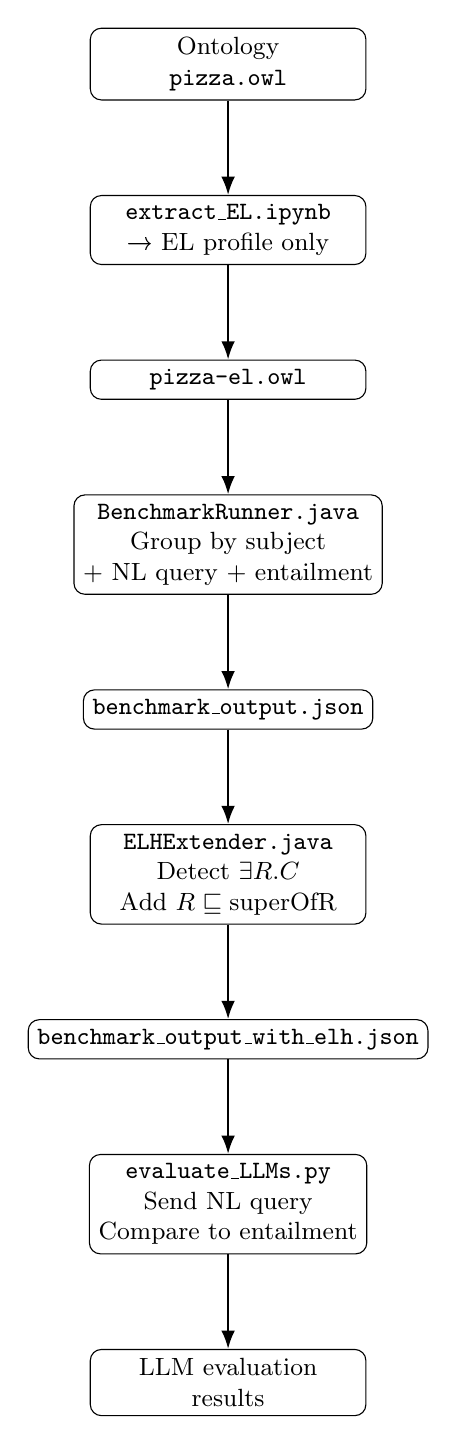
\begin{tikzpicture}[
        node distance=1.2cm and 2.5cm,
        every node/.style={draw, rounded corners, align=center, font=\small, minimum width=3.5cm},
        arrow/.style={-{Latex}, thick}
    ]

    \node (ont) {Ontology\\\texttt{pizza.owl}};
    \node (el) [below=of ont] {\texttt{extract\_EL.ipynb}\\→ EL profile only};
    \node (elowl) [below=of el] {\texttt{pizza-el.owl}};
    \node (bench) [below=of elowl] {\texttt{BenchmarkRunner.java}\\Group by subject\\+ NL query + entailment};
    \node (benchout) [below=of bench] {\texttt{benchmark\_output.json}};
    \node (elh) [below=of benchout] {\texttt{ELHExtender.java}\\Detect $\exists R.C$\\Add $R \sqsubseteq \text{superOfR}$};
    \node (elhout) [below=of elh] {\texttt{benchmark\_output\_with\_elh.json}};
    \node (eval) [below=of elhout] {\texttt{evaluate\_LLMs.py}\\Send NL query\\Compare to entailment};
    \node (res) [below=of eval] {LLM evaluation\\results};

    \draw [arrow] (ont) -- (el);
    \draw [arrow] (el) -- (elowl);
    \draw [arrow] (elowl) -- (bench);
    \draw [arrow] (bench) -- (benchout);
    \draw [arrow] (benchout) -- (elh);
    \draw [arrow] (elh) -- (elhout);
    \draw [arrow] (elhout) -- (eval);
    \draw [arrow] (eval) -- (res);

    \end{tikzpicture}
    \caption{Overview of the DL Reasoning Benchmarking Framework Pipeline}
    \label{fig:pipeline} 
\end{figure}

\newpage

The pipeline consists of four stages:

\begin{enumerate}
    \item \textbf{EL Ontology Extraction:} A subset of axioms conforming to the EL profile is extracted from the Pizza ontology using \texttt{extract\_EL.ipynb}. The output is an EL-compliant OWL file.
    
    \item \textbf{Benchmark Generation:} Java programs parse the EL ontology to group axioms by subject (\texttt{AxiomGrouper.java}), generate corresponding natural language queries (\texttt{QueryGenerator.java}), and compute ground-truth entailment using the HermiT reasoner (\texttt{ReasoningValidator.java}). These are saved in \texttt{benchmark\_output.json}.
    
    \item \textbf{ELH Extension:} The benchmark is enriched with role inclusion axioms to form ELH cases using \texttt{ELHExtender.java}, resulting in \texttt{benchmark\_output\_with\_elh.json}.
    
    \item \textbf{LLM Evaluation:} A Python script sends natural language queries to various LLMs (GPT-4o, Gemini, Gemma, LLaMA, etc.) using their APIs and compares their Yes/No predictions to ground-truth entailment.
\end{enumerate}

\subsection{DL Profiles and Scope}
The benchmark supports:
\begin{itemize}
    \item \textbf{EL:} A subset of DL supporting intersection and existential quantification
    \item \textbf{ELH:} EL extended with role hierarchy axioms (e.g., $r \sqsubseteq s$)
\end{itemize}
At this stage, no additional MR (metamorphic relation) types have been applied beyond the original EL/ELH logical transformations.

\subsection{Evaluation Metrics}
To ensure robust evaluation, each model was tested on the entire benchmark three times. Model performance is measured using the following metrics based on the aggregated results of these runs:

\begin{itemize}
    \item \textbf{Mean Accuracy:} The primary metric is the average accuracy across the three runs, representing the model's typical reasoning performance.
    
    \item \textbf{Consistency (Standard Deviation):} We report the standard deviation ($\sigma$) of the accuracy across the three runs. A low standard deviation indicates high consistency and reliability, while a high value suggests erratic performance.
    
    \item \textbf{Output Format Stability:} We track the number of correct responses that were not in the expected "Yes" or "No" format and required manual validation (e.g., answers embedded in a full sentence). This serves as a qualitative measure of the model's ability to follow instructions.
    
    \item \textbf{Execution Time and Errors:} We measure the total execution time and log any API failures or server errors encountered during the evaluation.
\end{itemize}

\newpage

\section{Results and Analysis}

We evaluated seven large language models on a benchmark dataset derived from the Pizza ontology. To ensure reliability, each model was evaluated three times. The aggregated results, covering accuracy, consistency, error patterns, and runtime performance, are presented in Table \ref{tab:performance_summary}.

\subsection{Overall Model Performance}

\begin{table}[htbp]
\centering
\small
\begin{threeparttable}
\caption{Model performance on EL and ELH. Accuracy values are reported as Mean $\pm$ Standard Deviation over three runs. Error counts are averages per run (ELH).}
\label{tab:performance_summary}
\begin{tabular}{lcccccc}
\toprule
Model & EL (\%) & ELH (\%) & FN & FP & Time & API \\
\midrule
GPT-4o                        & \textbf{100.0 $\pm$ 0.0} & \textbf{100.0 $\pm$ 0.0} & 0    & 0 & 45s     & 0 \\
Gemma 2 (4.3B Instruct)       & \textbf{100.0 $\pm$ 0.0} & 99.43 $\pm$ 0.99         & 0.33 & 0 & 22s     & 0 \\
Gemini 2.5 Pro                & 98.28 $\pm$ 0.0          & \textbf{100.0 $\pm$ 0.0} & 0.33 & 0 & 10+ min & 2 \\
Mistral (7B Instruct)         & 92.53 $\pm$ 2.65         & 96.55 $\pm$ 1.73         & 2    & 0 & 35s     & 0 \\
LLaMA 3 (8B Instruct)         & 83.33 $\pm$ 3.56         & 79.31 $\pm$ 4.49         & 12   & 0 & 30s     & 0 \\
Qwen 7B                       & 41.95 $\pm$ 2.00         & 30.46 $\pm$ 5.45         & 39   & 0 & 30s     & 0 \\
DeepSeek Coder (6.7B Instruct)& 14.94 $\pm$ 7.15         & 17.82 $\pm$ 9.81         & 45   & 0 & 4.5 min & 0 \\
\bottomrule
\end{tabular}
\begin{tablenotes}[flushleft]\footnotesize
\item EL = EL Accuracy; ELH = ELH Accuracy; FN = Avg. False Negatives; FP = Avg. False Positives; 
Time = wall-clock per run; API = API errors per run. Results averaged over three runs.
\end{tablenotes}
\end{threeparttable}
\end{table}

\subsection{Analysis of Results}
The results in Table \ref{tab:performance_summary} reveal a clear hierarchy of reasoning capabilities. 

\textbf{Accuracy and Consistency:} Top-tier models like \textbf{GPT-4o}, \textbf{Gemma 2}, and \textbf{Gemini 2.5 Pro} not only achieved the highest accuracy but also demonstrated exceptional consistency, with standard deviations at or near zero. In contrast, models like \textbf{LLaMA 3} and particularly \textbf{DeepSeek Coder} showed significant performance variability between runs, indicating a lack of stable reasoning processes.

\textbf{Error Analysis:} A crucial finding is the complete absence of \textbf{false positives} across all models. This suggests that the models, when they fail, do so by being overly cautious and failing to identify a valid entailment (a false negative), rather than inventing incorrect ones. The number of false negatives correlates directly with lower accuracy, with \textbf{LLaMA 3}, \textbf{Qwen 7B}, and \textbf{DeepSeek Coder} exhibiting a strong tendency to miss valid inferences.

\textbf{Practical Performance:} Practical usability diverges significantly. While highly accurate, \textbf{Gemini 2.5 Pro} suffered from extremely long execution times and was the only model to experience API stability issues (500 errors). Most other models offered rapid responses under a minute, with \textbf{Gemma 2} providing an excellent balance of top-tier accuracy, high consistency, and the fastest execution time.


\newpage

\subsection{Structural vs. HermiT Reasoner Runtime Comparison}

To establish a ground truth for entailment, we primarily used the well-established \textbf{HermiT} reasoner. For validation, we also compared its outputs against the OWL API's built-in \textbf{StructuralReasoner}. For all test cases in our EL benchmark, both reasoners produced identical entailment results, confirming the correctness of our ground truth. However, as shown in Table \ref{tab:reasoner-runtime}, their runtime performance differed substantially. This validates the use of either reasoner for the current scope while justifying HermiT’s role in future evaluations involving more complex logics.

\begin{table}[h!]
\centering
\caption{Average Runtime per Entailment Check (in nanoseconds)}
\label{tab:reasoner-runtime}
\begin{tabular}{|l|c|c|}
\hline
\textbf{Reasoner} & \textbf{Min Time (ns)} & \textbf{Max Time (ns)} \\
\hline
StructuralReasoner & 5,584 & 84,733 \\
HermiT Reasoner & 118,958 & 659,709 \\
\hline
\end{tabular}
\end{table}


The \textbf{StructuralReasoner}, which uses syntactic approximation and supports tractable fragments like EL, consistently achieved inference times under 20 microseconds. In contrast, \textbf{HermiT}, a complete tableau-based reasoner, required up to 660 microseconds due to its support for more expressive DLs and complete reasoning.

Despite the significant runtime gap, both reasoners agreed on all entailments in the EL test set. This agreement stems from the simplicity of the benchmark cases, which strictly conform to the OWL~2 EL profile—a fragment designed for efficient reasoning and fully supported by both systems.

This validates the use of StructuralReasoner for efficient EL benchmarking while justifying HermiT’s role in future evaluations involving more complex logics (e.g., ELH, ALC) or structural transformations under metamorphic testing.


\section{Conclusion and Future Work}
This study presents a comprehensive framework for benchmarking the reasoning capabilities of large language models (LLMs) using Description Logic (DL), specifically focusing on the EL and ELH fragments. By translating logical axioms into natural language queries and comparing model predictions against formal entailment results, we revealed substantial differences in model behavior, logical generalization, and sensitivity to DL complexity.

Our findings indicate GPT-4o, Gemma 2, and Gemini 2.5 Pro achieved consistently high accuracy and reliability in DL-style tasks. In contrast, LLaMA 3 and DeepSeek Coder exhibit significant deficiencies and performance instability, particularly in ELH settings.

Future work includes:
\begin{itemize}
    \item Implementing and evaluating more metamorphic reasoning types (e.g., paraphrasing, axiom removal)
    \item Expanding to additional DL fragments such as ALC or SHOIN
    \item Applying fine-tuning or prompt engineering to guide model reasoning more effectively
    \item Incorporating formal proof explanations alongside binary entailment responses
\end{itemize}

\newpage

\bibliographystyle{plain}
\bibliography{references}
\nocite{*}

\end{document}
